\documentclass[11pt]{article}

\usepackage[margin=1in]{geometry}
\usepackage[T1]{fontenc}
\usepackage[utf8]{inputenc}
\usepackage{amsmath,amssymb,amsthm,mathtools}
\usepackage{enumitem}
\usepackage{tikz}
\usetikzlibrary{arrows.meta,positioning}
\usepackage{hyperref}

\hypersetup{colorlinks=true, linkcolor=black, citecolor=black, urlcolor=black}

\newtheorem{definition}{Definition}
\newtheorem{lemma}{Lemma}
\newtheorem{theorem}{Theorem}

\newcommand{\E}{\mathbb{E}}
\newcommand{\Prb}{\mathbb{P}}
\newcommand{\ind}{\mathbf{1}}
\newcommand{\KT}{\operatorname{KT}}
\newcommand{\fas}{\operatorname{fas}}
\newcommand{\indeg}{\operatorname{indeg}}
\newcommand{\pos}{\operatorname{pos}}
\newcommand{\outdeg}{\operatorname{outdeg}}

\title{NP-Hardness of the Ordering Recovery Problem\\
\large Statement Summary and Dependency Diagram}
\author{}
\date{}

\begin{document}
\maketitle

\noindent
This document accompanies the main note \emph{NP-Hardness of the Ordering Recovery Problem: A Corrected and Simplified Reduction} and its companion appendix \emph{Auxiliary Lemmas} (\texttt{orp\_algebra\_appendix.pdf}).  It contains all definition, lemma, and theorem statements of the main note, with no proofs; the numbering of every statement matches the main note.  Statements are preceded only by the definitional setting they require.  The diagram below records which statement is used in the proof of which other statement.

\section{Dependency diagram}

Solid arrows are dependencies proved in the main note.  Dashed arrows are uses of the auxiliary lemmas A.1--A.15 from the companion appendix, labelled with the specific lemmas invoked.  Lemma~3 (profile construction) is stated entirely in terms of the arc gadgets of Definition~3, so the diagram shows the statement-level dependency Definition~3 $\to$ Lemma~3; the bijectivity and combinatorial properties of the gadget position maps are stated and proved in the companion appendix as Lemma~A.15.  The objective identity, previously derived inline in Section~3.6 of the main note, is now stated as Theorem~1 (equation~\eqref{eq:objective-identity} below).  ``FAST is NP-complete'' is an external input cited from the literature.

\begin{center}
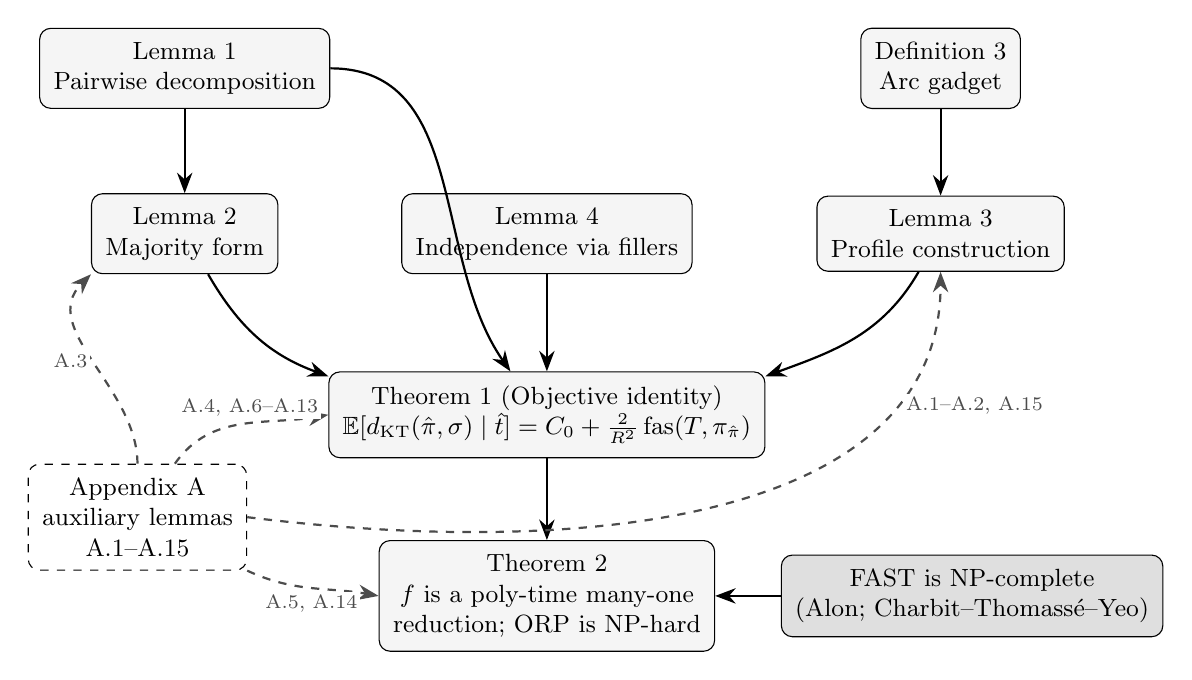
\begin{tikzpicture}[
  stmt/.style={draw, rounded corners, align=center, fill=gray!8,
               minimum height=9mm, inner sep=5pt, font=\small},
  ext/.style={draw, rounded corners, align=center, fill=gray!25,
              minimum height=9mm, inner sep=5pt, font=\small},
  app/.style={draw, dashed, rounded corners, align=center, fill=white,
              minimum height=9mm, inner sep=5pt, font=\small},
  dep/.style={-{Stealth[length=2.6mm]}, thick},
  adep/.style={-{Stealth[length=2.6mm]}, thick, dashed, gray!60!black},
  lab/.style={font=\scriptsize, fill=white, inner sep=1pt, text=gray!60!black}
]
  % Row 1
  \node[stmt] (L1) at (1.0,7.6)  {Lemma 1\\ Pairwise decomposition};
  \node[stmt] (D3) at (10.6,7.6) {Definition 3\\ Arc gadget};
  % Row 2
  \node[stmt] (L2) at (1.0,5.5)  {Lemma 2\\ Majority form};
  \node[stmt] (L5) at (5.6,5.5)  {Lemma 4\\ Independence via fillers};
  \node[stmt] (L4) at (10.6,5.5) {Lemma 3\\ Profile construction};
  % Row 3
  \node[stmt] (OI) at (5.6,3.2)
    {Theorem 1 (Objective identity)\\
     $\E[d_{\KT}(\hat\pi,\sigma)\mid\hat t]=C_0+\frac{2}{R^2}\fas(T,\pi_{\hat\pi})$};
  % Row 4
  \node[stmt] (TH) at (5.6,0.9)  {Theorem 2\\ $f$ is a poly-time many-one\\ reduction; ORP is NP-hard};
  \node[ext]  (FA) at (11.0,0.9) {FAST is NP-complete\\ (Alon; Charbit--Thomass\'e--Yeo)};
  % Appendix node
  \node[app]  (AP) at (0.4,1.9)  {Appendix A\\ auxiliary lemmas\\ A.1--A.15};

  % Main-note dependencies
  \draw[dep] (L1) -- (L2);
  \draw[dep] (D3) -- (L4);
  \draw[dep] (L1.east) to[out=0,in=125] (OI.130);
  \draw[dep] (L2) to[out=-60,in=160] (OI.170);
  \draw[dep] (L5) -- (OI);
  \draw[dep] (L4) to[out=-120,in=20] (OI.10);
  \draw[dep] (OI) -- (TH);
  \draw[dep] (FA) -- (TH);

  % Appendix dependencies (dashed, labelled)
  \draw[adep] (AP.north) to[out=90,in=-135] node[lab, pos=0.5, left=1pt] {A.3} (L2.south west);
  \draw[adep] (AP.east) .. controls (6.2,1.35) and (10.6,1.9) .. (L4.south)
      node[lab, pos=0.78, right=3pt] {A.1--A.2, A.15};
  \draw[adep] (AP.55)    to[out=55,in=-170] node[lab, pos=0.55, above=1pt] {A.4, A.6--A.13} (OI.west);
  \draw[adep] (AP.south east) to[out=-25,in=170] node[lab, pos=0.5, below=1pt] {A.5, A.14} (TH.west);
\end{tikzpicture}
\end{center}

\noindent
Reading guide: Lemma~2's proof uses Lemma~1 and the max--min decomposition A.3.  Lemma~3's proof combines the gadget position properties A.15 with the summation identities A.1--A.2.  Theorem~1 (the objective identity) combines the pairwise decomposition (Lemma~1), the majority form (Lemma~2), the profile counts and rank sums (Lemma~3), and posterior independence (Lemma~4), with the algebra A.4 and A.6--A.13 carrying the intermediate computations.  Theorem~2 states the reduction $f$ explicitly (its statement references the profile of Lemma~3 and the instance construction) and follows from Theorem~1 via the threshold equivalence A.14, with instance well-formedness supplied by A.5 ($\alpha_u\in(0,1)$) and NP-completeness of FAST supplied by the literature.  Internally to the appendix, A.4 uses A.3 and A.9 uses A.6; A.15 stands alone.

\section{Preliminaries}

We write $S_L$ for the symmetric group on $\{1,\ldots,L\}$.  A permutation $\pi\in S_L$ is interpreted as a ranking: $\pi(i)$ is the position assigned to item $i$, and item $i$ precedes item $j$ when $\pi(i)<\pi(j)$.

\begin{definition}[Minimum Feedback Arc Set in Tournaments]
A tournament is a directed graph $T=(V,A)$ such that for every unordered pair $\{u,v\}\subseteq V$ exactly one of $(u,v)$ and $(v,u)$ is in $A$.  For a linear order $\pi$ of $V$, define
\begin{equation}
  \fas(T,\pi)=\left|\{(u,v)\in A: \pi(u)>\pi(v)\}\right| .
\end{equation}
The FAST decision problem asks, given a tournament $T$ and an integer $k\ge 0$, whether there exists a linear order $\pi$ of $V$ with $\fas(T,\pi)\le k$.  FAST is NP-complete \cite{Alon2006,Charbit2007}.
\end{definition}

\begin{definition}[Ordering Recovery Problem]
An ORP instance has $L$ events $e_1,\ldots,e_L$.  A hidden permutation $\sigma\in S_L$ is drawn uniformly at random, and event $e_i$ occupies slot $\sigma(i)$, giving it true timestamp
\begin{equation}
  t_i^*=\sigma(i)\Delta,
\end{equation}
where $\Delta>0$ is fixed.  The observation is
\begin{equation}
  \hat t_i=t_i^*+\eta_i,
\end{equation}
where the noise variables $\eta_i\sim F_i$ are mutually independent and independent of $\sigma$.  In this note the distributions $F_i$ are finite-support rational probability mass functions.

Given the observation vector $\hat t=(\hat t_1,\ldots,\hat t_L)$ and a candidate output order $\hat\pi\in S_L$, the loss is the posterior expected Kendall-tau distance
\begin{equation}
  \E\left[d_{\KT}(\hat\pi,\sigma)\mid \hat t\right],
\end{equation}
where
\begin{equation}
  d_{\KT}(\hat\pi,\sigma)
  =\sum_{i<j}
  \ind\!\big[(\sigma(i)-\sigma(j))(\hat\pi(i)-\hat\pi(j))<0\big].
\end{equation}
The ORP decision problem asks whether there exists $\hat\pi\in S_L$ with
\begin{equation}
  \E\left[d_{\KT}(\hat\pi,\sigma)\mid \hat t\right]\le K,
\end{equation}
where $K$ is a non-negative rational threshold.
\end{definition}

\section{Pairwise decomposition}

\begin{lemma}[Pairwise decomposition]\label{lem:pairwise}
For any prior distribution on $\sigma\in S_L$ and any observation vector $\hat t$,
\begin{align}
  \E\left[d_{\KT}(\hat\pi,\sigma)\mid \hat t\right]
  =\sum_{i<j} &\Prb(\sigma(i)<\sigma(j)\mid \hat t)\,\ind[\hat\pi(i)>\hat\pi(j)] \notag\\
  &+\Prb(\sigma(i)>\sigma(j)\mid \hat t)\,\ind[\hat\pi(i)<\hat\pi(j)].
\end{align}
\end{lemma}

\begin{lemma}[Majority form of a pairwise contribution]\label{lem:majority}
Fix $i<j$ and write
\begin{equation}
  p_{ij}=\Prb(\sigma(i)<\sigma(j)\mid \hat t).
\end{equation}
Call the more likely relative order the posterior majority order, breaking ties arbitrarily.  The contribution of pair $\{i,j\}$ to the posterior expected Kendall-tau distance is
\begin{equation}
  |2p_{ij}-1|\,\ind[\hat\pi\text{ disagrees with the posterior majority order on }\{i,j\}]
  +\min(p_{ij},1-p_{ij}).
\end{equation}
In particular, if $p_{ij}=1/2$, the contribution is always $1/2$, independent of $\hat\pi$.
\end{lemma}

\section{The reduction: statements}

Throughout, $(T,k)$ is a FAST instance with $T=(V,A)$ a tournament on $V=\{1,\ldots,n\}$, $m=\binom n2$, and $\delta_u=\indeg(u)-\outdeg(u)$ for $u\in V$; instances with $n\le 3$ are decided by brute force, so $n\ge 4$ is assumed.  For linear orders $\rho_1,\ldots,\rho_R$ of $V$ and an ordered pair $u\ne v$, $c_{uv}=|\{b:\rho_b(u)<\rho_b(v)\}|$ denotes the number of orders ranking $u$ before $v$.

\begin{definition}[Arc gadget]\label{def:gadget}
For a linear order $O$ of $V$ and $w\in V$, write $\pos_O(w)\in\{1,\ldots,n\}$ for the position of $w$ in $O$.  Let $(u,v)\in A$ and fix an arbitrary enumeration $x_1,\ldots,x_{n-2}$ of $V\setminus\{u,v\}$.  The \emph{gadget pair} of the arc $(u,v)$ is the pair of linear orders
\begin{equation}
  O_1=(u,\,v,\,x_1,\ldots,x_{n-2}),\qquad
  O_2=(x_{n-2},\ldots,x_1,\,u,\,v),
\end{equation}
that is, the orders defined by the position formulas
\begin{equation}\label{eq:gadget-positions}
\begin{aligned}
  \pos_{O_1}(u)&=1, & \pos_{O_1}(v)&=2, & \pos_{O_1}(x_j)&=2+j &&(1\le j\le n-2),\\
  \pos_{O_2}(u)&=n-1, & \pos_{O_2}(v)&=n, & \pos_{O_2}(x_j)&=n-1-j &&(1\le j\le n-2).
\end{aligned}
\end{equation}
By Lemma~A.15 of the companion appendix, applied with the symbols $u,v$ and the chosen enumeration $x_1,\ldots,x_{n-2}$ of $V\setminus\{u,v\}$, each row of \eqref{eq:gadget-positions} is a bijection $V\to\{1,\ldots,n\}$, so $O_1$ and $O_2$ are indeed linear orders of $V$.
\end{definition}

\begin{lemma}[Profile construction]\label{lem:profile}
Set $R=2m=n(n-1)$, an even integer.  Enumerate the arcs as $A=\{a_1,\ldots,a_m\}$ and define the \emph{profile} to be the sequence of linear orders
\begin{equation}
  \rho_1,\ldots,\rho_R
\end{equation}
of $V$ obtained by letting $(\rho_{2c-1},\rho_{2c})$ be the gadget pair of arc $a_c$ from Definition~\ref{def:gadget}, for $c=1,\ldots,m$; as before, $\rho_b(u)$ denotes the rank position of $u$ in order $\rho_b$.  The profile is constructible in polynomial time and satisfies:
\begin{enumerate}[label=(\roman*)]
\item for every ordered pair $u\ne v$, if $(u,v)\in A$ then
\begin{equation}
  c_{uv}=\frac R2+1,
\end{equation}
and if $(v,u)\in A$ then
\begin{equation}
  c_{uv}=\frac R2-1;
\end{equation}
\item for every vertex $u$,
\begin{equation}
  \sum_{b=1}^R \rho_b(u)=\frac{R(n+1)}2+\delta_u.
\end{equation}
\end{enumerate}
\end{lemma}

\subsection*{The ORP instance (construction)}

Set $L=2nR$ and $q=L-n$.  The instance has one designated event $d_u$ per vertex $u\in V$ and $q$ filler events; $\Delta=1$ and every observation is $\hat t_i=0$.  The $L$ slots form $R$ consecutive blocks of width $2n$; for vertex $u$ and block $b$, the consecutive slot pair is
\begin{equation}
  a^-_{u,b}=(b-1)2n+2\rho_b(u)-1,\qquad a^+_{u,b}=(b-1)2n+2\rho_b(u).
\end{equation}
With
\begin{equation}
  \alpha_u=\frac12-\frac{2\delta_u}{R}+\frac{\delta_u}{R^2}\;\in(0,1),
\end{equation}
the designated noise distribution puts mass $(1-\alpha_u)/R$ on $-a^-_{u,b}$ and $\alpha_u/R$ on $-a^+_{u,b}$ for each block $b$, and each filler has the uniform noise distribution with mass $1/L$ on $-s$ for $s=1,\ldots,L$.  We write $X_u$ for the slot occupied by $d_u$ under the posterior given $\hat t$.

\begin{lemma}[Independence via fillers]
Conditioned on the observation vector, the slots of the designated events are mutually independent.  More precisely,
\begin{equation}
  \Prb(X_u=a_{u,b}^-\mid \hat t)=\frac{1-\alpha_u}{R},
  \qquad
  \Prb(X_u=a_{u,b}^+\mid \hat t)=\frac{\alpha_u}{R},
\end{equation}
where $X_u$ is the slot occupied by $d_u$.
\end{lemma}

\subsection*{The objective identity}

Let
\begin{equation}
  C_0=m\left(\frac12-\frac1{R^2}\right)+\left(\binom L2-m\right)\frac12,
\end{equation}
and for $\hat\pi\in S_L$ let $\pi_{\hat\pi}$ be the induced vertex order: $\pi_{\hat\pi}(u)<\pi_{\hat\pi}(v)\iff\hat\pi(d_u)<\hat\pi(d_v)$.

\begin{theorem}[Objective identity]\label{thm:objident}
For every $\hat\pi\in S_L$,
\begin{equation}
  \E\left[d_{\KT}(\hat\pi,\sigma)\mid \hat t\right]
  =C_0+\frac2{R^2}\fas(T,\pi_{\hat\pi}).
  \label{eq:objective-identity}
\end{equation}
\end{theorem}

\begin{theorem}
Let $(T,k)$ be a FAST instance on vertex set $V=\{1,\ldots,n\}$ with $n\ge 4$, and let $f(T,k)$ be the ORP instance constructed above from the profile $\rho_1,\ldots,\rho_R$ of Lemma~\ref{lem:profile}: $L=2nR$ events comprising one designated event $d_u$ per vertex $u\in V$, with noise distribution $F_{d_u}$ supported on the slot pairs $a^{\pm}_{u,b}$ with weights $(1-\alpha_u)/R$ and $\alpha_u/R$, and $q=L-n$ filler events with uniform noise, all observations equal to zero, together with the threshold $K=C_0+2k/R^2$.  Then $f$ is computable in deterministic polynomial time and
\begin{equation}
  (T,k)\in\mathrm{FAST}
  \quad\Longleftrightarrow\quad
  f(T,k)\in\mathrm{ORP}.
\end{equation}
In particular, the Ordering Recovery Problem is NP-hard under deterministic polynomial-time many-one reductions.
\end{theorem}

\end{document}
